\section{Architettura del sistema}
DermaTriage è un sistema di triage dermatologico assistito da intelligenza
artificiale, sviluppato nell'ambito del progetto AI vs Cancer. Il sistema
elabora immagini di lesioni cutanee inviate dai pazienti insieme a
informazioni cliniche e demografiche, con l'obiettivo di stimare il livello
di urgenza del caso e assegnare una priorità clinica compresa tra P1 e P4.

DermaTriage è integrato con la piattaforma B4 (Social Things), che rappresenta
il punto di interazione con il paziente e mette a disposizione le API utilizzate
per lo scambio dei dati relativi ai consulti, ai documenti caricati, ai risultati
diagnostici e alle validazioni mediche. L'elaborazione diagnostica viene invece
eseguita dal servizio DermaTriage, che espone un'applicazione FastAPI e implementa
una pipeline di intelligenza artificiale composta da quattro stadi, seguita da
un adaptation layer responsabile della conversione del risultato nella scala
clinica P1-P4.

\subsection{Ambito del sistema e integrazione con B4}
L'interazione con il paziente avviene attraverso la piattaforma B4, che
raccoglie le informazioni necessarie per avviare il processo di triage.
Nel flusso principale vengono acquisiti un'immagine della lesione cutanea,
l'età del paziente, il sesso e la localizzazione anatomica della lesione.
A questi dati possono aggiungersi informazioni relative alla sintomatologia,
tra cui prurito, sanguinamento, crescita della lesione, cambiamenti
morfologici e dolore.

Una volta raccolti i dati, DermaTriage accede alle informazioni associate
alla richiesta attraverso le API messe a disposizione da B4. Il servizio
può recuperare le pratiche disponibili, individuare i documenti associati
e scaricare l'immagine dermatologica necessaria all'elaborazione. Al termine
della pipeline diagnostica, il risultato viene restituito a B4 e associato
alla relativa richiesta di triage. La successiva validazione da parte del
personale medico permette di ottenere un riscontro sull'esito prodotto dal
sistema. Tali informazioni possono essere recuperate da DermaTriage e
utilizzate come feedback per l'evoluzione dei prompt e per il retraining
del classificatore EfficientNet-B4.

La comunicazione tra DermaTriage e B4 avviene tramite API REST protette da
autenticazione. L'accesso ai servizi B4 utilizza un Bearer JWT ottenuto
tramite l'endpoint \texttt{/api/v1/auth/token}; la gestione del token è
affidata al componente \texttt{B4Auth}, che ne esegue il rinnovo automatico
alla scadenza. I parametri necessari all'integrazione, tra cui credenziali,
API key e indirizzo del servizio B4, sono configurati mediante variabili
d'ambiente dedicate.

Il flusso integrato viene avviato attraverso l'endpoint
\texttt{POST /diagnose}, al quale viene fornito un
\texttt{consulto\_id} come riferimento alla richiesta da elaborare.
L'accesso a questo endpoint richiede l'header \texttt{X-API-Key}, utilizzato
anche per le funzionalità amministrative relative alla validazione delle
diagnosi, alla gestione dei prompt e al retraining dei modelli.

Accanto al percorso integrato con B4, DermaTriage espone anche
\texttt{POST /analyze}, che permette di avviare direttamente la pipeline
fornendo un'immagine JPEG o PNG insieme a età, sesso e localizzazione.
Questo secondo percorso consente quindi di utilizzare il motore diagnostico
anche senza partire da una richiesta già presente sulla piattaforma B4.

Dal punto di vista architetturale, B4 e DermaTriage mantengono ruoli distinti.
B4 gestisce l'interazione iniziale con il paziente e rende disponibili i dati
necessari al processo di triage, mentre DermaTriage esegue l'elaborazione
diagnostica e gestisce i meccanismi di aggiornamento dei modelli.
L'integrazione tra i due sistemi è quindi bidirezionale e accompagna il caso
clinico dalla fase di acquisizione fino alla restituzione e alla successiva
validazione del risultato.

\subsection{Pipeline di elaborazione e decisione clinica}
L'elaborazione interna di DermaTriage segue una sequenza di quattro stadi,
ognuno dei quali produce informazioni utilizzate nelle fasi successive.
L'architettura combina un classificatore visuale, un modello
vision-language, un sistema di retrieval basato su casi clinici e un modello
linguistico specializzato in ambito medico. Il risultato ottenuto al termine
di questi passaggi viene successivamente trasformato nella priorità clinica
utilizzata dal sistema.

\subsubsection{Stage 1 - Classificazione dell'urgenza con EfficientNet-B4}
Il primo stadio esegue una classificazione dell'immagine della lesione
attraverso EfficientNet-B4, un modello convoluzionale sottoposto a
fine-tuning per distinguere tre livelli di urgenza denominati
\texttt{HIGH}, \texttt{MEDIUM} e \texttt{LOW}. L'immagine viene elaborata
come input RGB di dimensione $380 \times 380$ pixel e il modello restituisce,
oltre alla classe prevista, un valore di confidenza e le probabilità
associate alle tre classi.

Per aumentare la sensibilità verso i casi considerati più urgenti,
la classificazione \texttt{HIGH} utilizza una soglia operativa pari a
$0.25$. Questa prima valutazione non determina direttamente la priorità
finale P1--P4, ma costituisce una delle informazioni utilizzate nelle fasi
successive della pipeline.

\subsubsection{Stage 2 - Descrizione clinica con Qwen2-VL}
In parallelo alla classificazione dell'urgenza, l'immagine viene analizzata
da Qwen2-VL-7B-Instruct. Il modello interpreta visivamente la lesione e
genera una descrizione clinica testuale organizzata in cinque aspetti
principali, relativi alla forma, ai bordi, al colore, alla texture e alla
presenza di caratteristiche considerate sospette.

Questo passaggio trasforma quindi il contenuto visuale in una
rappresentazione testuale strutturata. La descrizione prodotta non rappresenta
ancora una decisione diagnostica, ma viene utilizzata come query per la fase
di ricerca dei casi clinici simili.

\subsubsection{Stage 3 - Recupero di casi clinici simili}
Il terzo stadio introduce un meccanismo di Retrieval-Augmented Generation
basato su ChromaDB. La descrizione generata da Qwen2-VL viene convertita in
una rappresentazione vettoriale mediante il modello
\texttt{all-MiniLM-L6-v2} e confrontata con le descrizioni presenti
nell'indice vettoriale.

La ricerca utilizza la similarità coseno e seleziona i cinque casi più
vicini alla descrizione della lesione corrente. Per ciascun risultato vengono
recuperate informazioni quali l'identificativo anonimizzato del paziente,
la diagnosi associata, il livello di urgenza e il punteggio di similarità.
In questo modo la pipeline affianca alla valutazione dell'immagine un
riferimento a casi clinici precedenti con caratteristiche semanticamente
simili.

\subsubsection{Stage 4 - Sintesi clinica con BioMistral}
Le informazioni prodotte nei primi tre stadi vengono successivamente
aggregate e fornite a BioMistral-7B insieme ai dati relativi alla
sintomatologia del paziente. Il modello riceve quindi la classificazione
prodotta da EfficientNet-B4, la descrizione visuale generata da Qwen2-VL
e i casi recuperati dal sistema RAG, disponendo di un contesto più ampio
rispetto a quello disponibile nei singoli stadi precedenti.

BioMistral produce una risposta strutturata contenente il livello finale di
urgenza, la relativa confidenza, una motivazione della decisione,
l'azione raccomandata e una possibile patologia associata. Questo risultato
rappresenta l'uscita della componente di inferenza vera e propria e viene
successivamente elaborato dall'adaptation layer.

\subsubsection{Adaptation layer e assegnazione della priorità}
L'adaptation layer converte il livello di urgenza prodotto dalla pipeline
nella scala P1--P4 utilizzata per il triage. La funzione
\texttt{map\_urgency\_to\_p\_scale()} applica una serie di regole che tengono
conto sia della classe di urgenza sia, per i casi \texttt{HIGH}, del livello
di confidenza ottenuto.

Un risultato \texttt{HIGH} con confidenza superiore a $0.85$ viene associato
alla priorità P1, con un tempo previsto di presa in carico pari a 24 ore.
Gli altri casi \texttt{HIGH} vengono assegnati a P2 con un intervallo di
48 ore, mentre le classi \texttt{MEDIUM} e \texttt{LOW} vengono convertite
rispettivamente in P3, con 72 ore, e P4, con 7 giorni.

L'output finale comprende quindi la priorità P1-P4, il livello di confidenza,
lo specialista indicato e il relativo SLA. L'adaptation layer separa in questo
modo il risultato interno prodotto dai modelli dalla rappresentazione
utilizzata per il triage clinico.

La Figura~\ref{fig:architettura-dermatriage} riassume i principali componenti
dell'architettura e il percorso seguito dalle informazioni durante
l'elaborazione di una richiesta di triage.

\begin{figure}[ht]
  \centering
  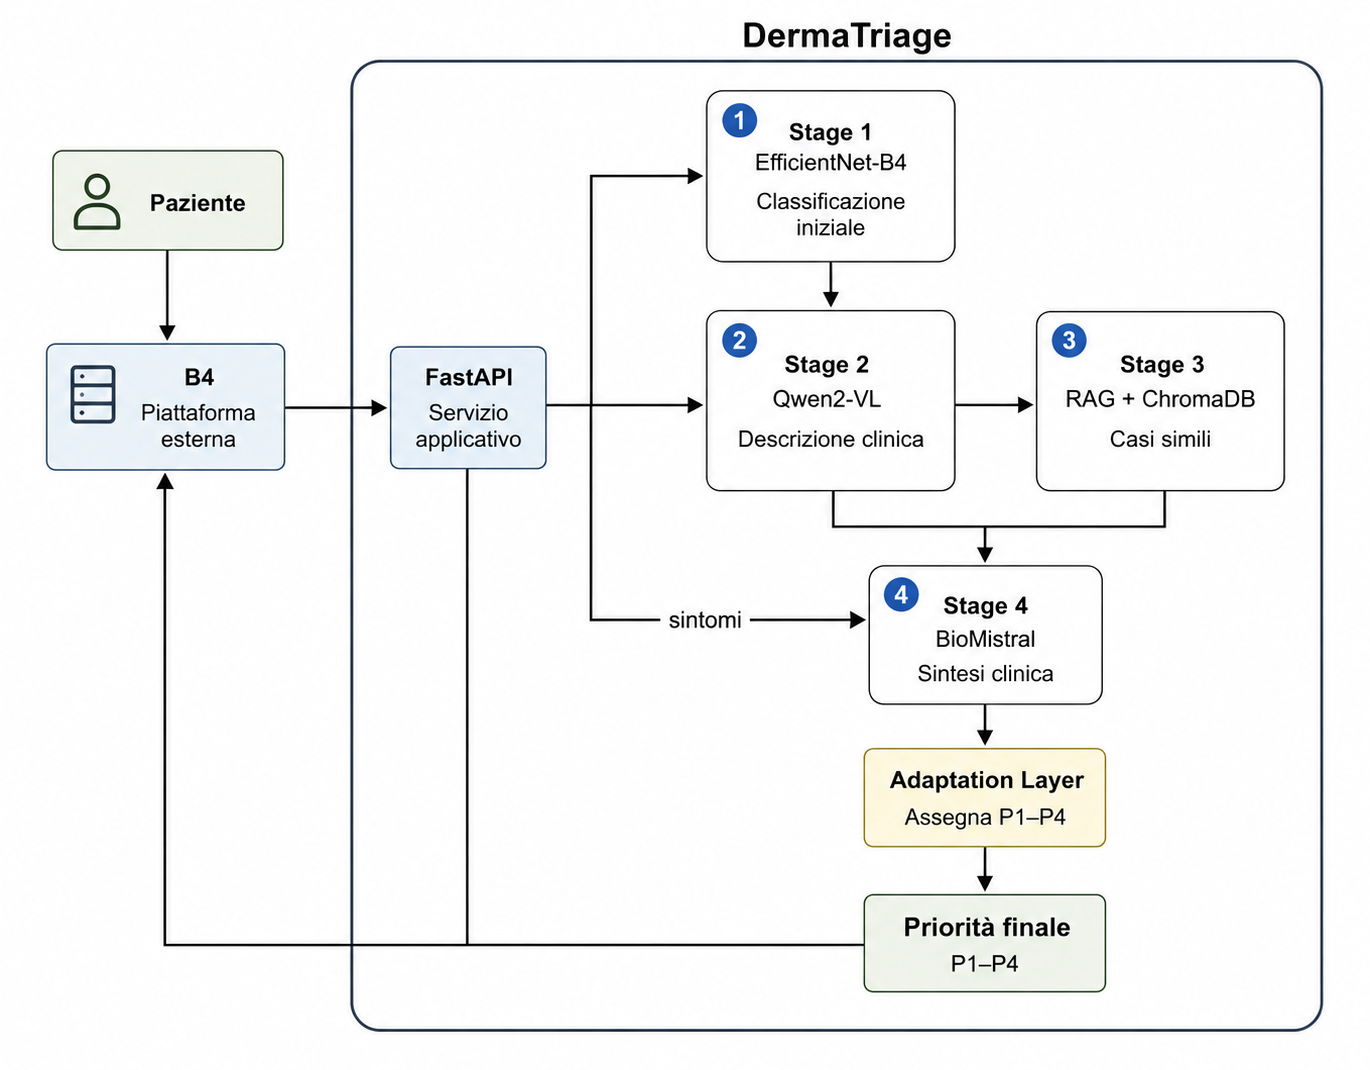
\includegraphics[width=0.85\linewidth]{../Immagini/Architettura del sistema.png}
  \caption{Architettura logica di DermaTriage e flusso principale di elaborazione}
  \label{fig:architettura-dermatriage}
\end{figure}